\documentclass[a4paper]{book}
\usepackage{makeidx}
\usepackage{graphicx}
\usepackage{multicol}
\usepackage{float}
\usepackage{listings}
\usepackage{color}
\usepackage{ifthen}
\usepackage[table]{xcolor}
\usepackage{textcomp}
\usepackage{alltt}
\usepackage{ifpdf}
\ifpdf
\usepackage[pdftex,
            pagebackref=true,
            colorlinks=true,
            linkcolor=blue,
            unicode
           ]{hyperref}
\else
\usepackage[ps2pdf,
            pagebackref=true,
            colorlinks=true,
            linkcolor=blue,
            unicode
           ]{hyperref}
\usepackage{pspicture}
\fi
\usepackage[utf8]{inputenc}
\usepackage{mathptmx}
\usepackage[scaled=.90]{helvet}
\usepackage{courier}
\usepackage{sectsty}
\usepackage[titles]{tocloft}
\usepackage{doxygen}
\lstset{language=C++,inputencoding=utf8,basicstyle=\footnotesize,breaklines=true,breakatwhitespace=true,tabsize=8,numbers=left }
\makeindex
\setcounter{tocdepth}{3}
\renewcommand{\footrulewidth}{0.4pt}
\renewcommand{\familydefault}{\sfdefault}
\begin{document}
\hypersetup{pageanchor=false}
\begin{titlepage}
\vspace*{7cm}
\begin{center}
{\Large Machine Learning Package }\\
\vspace*{1cm}
{\large Generated by Doxygen 1.7.4}\\
\vspace*{0.5cm}
{\small Wed Jun 1 2011 21:38:07}\\
\end{center}
\end{titlepage}
\clearemptydoublepage
\pagenumbering{roman}
\tableofcontents
\clearemptydoublepage
\pagenumbering{arabic}
\hypersetup{pageanchor=true}
\chapter{Class Index}
\section{Class Hierarchy}
This inheritance list is sorted roughly, but not completely, alphabetically:\begin{DoxyCompactList}
\item \contentsline{section}{mlpack::DataIndexer}{\pageref{classmlpack_1_1_data_indexer}}{}
\begin{DoxyCompactList}
\item \contentsline{section}{mlpack::BaseDataIndexer}{\pageref{classmlpack_1_1_base_data_indexer}}{}
\begin{DoxyCompactList}
\item \contentsline{section}{mlpack::OnePassDataIndexer}{\pageref{classmlpack_1_1_one_pass_data_indexer}}{}
\end{DoxyCompactList}
\end{DoxyCompactList}
\item \contentsline{section}{mlpack::Event}{\pageref{structmlpack_1_1_event}}{}
\item \contentsline{section}{mlpack::EventStream}{\pageref{classmlpack_1_1_event_stream}}{}
\begin{DoxyCompactList}
\item \contentsline{section}{mlpack::FileBasedEventStream}{\pageref{classmlpack_1_1_file_based_event_stream}}{}
\begin{DoxyCompactList}
\item \contentsline{section}{mlpack::FileEventStream}{\pageref{classmlpack_1_1_file_event_stream}}{}
\begin{DoxyCompactList}
\item \contentsline{section}{mlpack::RealValueFileEventStream}{\pageref{classmlpack_1_1_real_value_file_event_stream}}{}
\end{DoxyCompactList}
\item \contentsline{section}{mlpack::PredicateEventStream}{\pageref{classmlpack_1_1_predicate_event_stream}}{}
\begin{DoxyCompactList}
\item \contentsline{section}{mlpack::RealPredicateEventStream}{\pageref{classmlpack_1_1_real_predicate_event_stream}}{}
\end{DoxyCompactList}
\end{DoxyCompactList}
\item \contentsline{section}{mlpack::SequenceEventStream}{\pageref{classmlpack_1_1_sequence_event_stream}}{}
\end{DoxyCompactList}
\item \contentsline{section}{mlpack::Feature}{\pageref{structmlpack_1_1_feature}}{}
\item \contentsline{section}{mlpack::FeatureSet}{\pageref{structmlpack_1_1_feature_set}}{}
\item \contentsline{section}{mlpack::MaxentParameters}{\pageref{classmlpack_1_1_maxent_parameters}}{}
\item \contentsline{section}{mlpack::Model}{\pageref{classmlpack_1_1_model}}{}
\begin{DoxyCompactList}
\item \contentsline{section}{mlpack::GISModel}{\pageref{classmlpack_1_1_g_i_s_model}}{}
\end{DoxyCompactList}
\item \contentsline{section}{mlpack::Parameters}{\pageref{classmlpack_1_1_parameters}}{}
\item \contentsline{section}{mlpack::Prior}{\pageref{classmlpack_1_1_prior}}{}
\begin{DoxyCompactList}
\item \contentsline{section}{mlpack::UniformPrior}{\pageref{classmlpack_1_1_uniform_prior}}{}
\end{DoxyCompactList}
\item \contentsline{section}{mlpack::Trainer$<$ T $>$}{\pageref{classmlpack_1_1_trainer}}{}
\item \contentsline{section}{mlpack::Trainer$<$ GISModel $>$}{\pageref{classmlpack_1_1_trainer}}{}
\begin{DoxyCompactList}
\item \contentsline{section}{mlpack::GISTrainer}{\pageref{classmlpack_1_1_g_i_s_trainer}}{}
\end{DoxyCompactList}
\end{DoxyCompactList}

\chapter{Class Index}
\section{Class List}
Here are the classes, structs, unions and interfaces with brief descriptions:\begin{DoxyCompactList}
\item\contentsline{section}{\hyperlink{classmlpack_1_1_base_data_indexer}{mlpack::BaseDataIndexer} }{\pageref{classmlpack_1_1_base_data_indexer}}{}
\item\contentsline{section}{\hyperlink{classmlpack_1_1_data_indexer}{mlpack::DataIndexer} }{\pageref{classmlpack_1_1_data_indexer}}{}
\item\contentsline{section}{\hyperlink{structmlpack_1_1_event}{mlpack::Event} }{\pageref{structmlpack_1_1_event}}{}
\item\contentsline{section}{\hyperlink{classmlpack_1_1_event_stream}{mlpack::EventStream} }{\pageref{classmlpack_1_1_event_stream}}{}
\item\contentsline{section}{\hyperlink{structmlpack_1_1_feature}{mlpack::Feature} }{\pageref{structmlpack_1_1_feature}}{}
\item\contentsline{section}{\hyperlink{structmlpack_1_1_feature_set}{mlpack::FeatureSet} }{\pageref{structmlpack_1_1_feature_set}}{}
\item\contentsline{section}{\hyperlink{classmlpack_1_1_file_based_event_stream}{mlpack::FileBasedEventStream} }{\pageref{classmlpack_1_1_file_based_event_stream}}{}
\item\contentsline{section}{\hyperlink{classmlpack_1_1_file_event_stream}{mlpack::FileEventStream} }{\pageref{classmlpack_1_1_file_event_stream}}{}
\item\contentsline{section}{\hyperlink{classmlpack_1_1_g_i_s_model}{mlpack::GISModel} }{\pageref{classmlpack_1_1_g_i_s_model}}{}
\item\contentsline{section}{\hyperlink{classmlpack_1_1_g_i_s_trainer}{mlpack::GISTrainer} }{\pageref{classmlpack_1_1_g_i_s_trainer}}{}
\item\contentsline{section}{\hyperlink{classmlpack_1_1_maxent_parameters}{mlpack::MaxentParameters} }{\pageref{classmlpack_1_1_maxent_parameters}}{}
\item\contentsline{section}{\hyperlink{classmlpack_1_1_model}{mlpack::Model} }{\pageref{classmlpack_1_1_model}}{}
\item\contentsline{section}{\hyperlink{classmlpack_1_1_one_pass_data_indexer}{mlpack::OnePassDataIndexer} }{\pageref{classmlpack_1_1_one_pass_data_indexer}}{}
\item\contentsline{section}{\hyperlink{classmlpack_1_1_parameters}{mlpack::Parameters} }{\pageref{classmlpack_1_1_parameters}}{}
\item\contentsline{section}{\hyperlink{classmlpack_1_1_predicate_event_stream}{mlpack::PredicateEventStream} }{\pageref{classmlpack_1_1_predicate_event_stream}}{}
\item\contentsline{section}{\hyperlink{classmlpack_1_1_prior}{mlpack::Prior} }{\pageref{classmlpack_1_1_prior}}{}
\item\contentsline{section}{\hyperlink{classmlpack_1_1_real_predicate_event_stream}{mlpack::RealPredicateEventStream} }{\pageref{classmlpack_1_1_real_predicate_event_stream}}{}
\item\contentsline{section}{\hyperlink{classmlpack_1_1_real_value_file_event_stream}{mlpack::RealValueFileEventStream} }{\pageref{classmlpack_1_1_real_value_file_event_stream}}{}
\item\contentsline{section}{\hyperlink{classmlpack_1_1_sequence_event_stream}{mlpack::SequenceEventStream} }{\pageref{classmlpack_1_1_sequence_event_stream}}{}
\item\contentsline{section}{\hyperlink{classmlpack_1_1_trainer}{mlpack::Trainer$<$ T $>$} }{\pageref{classmlpack_1_1_trainer}}{}
\item\contentsline{section}{\hyperlink{classmlpack_1_1_uniform_prior}{mlpack::UniformPrior} }{\pageref{classmlpack_1_1_uniform_prior}}{}
\end{DoxyCompactList}

\chapter{Class Documentation}
\hypertarget{classmlpack_1_1_base_data_indexer}{
\section{mlpack::BaseDataIndexer Class Reference}
\label{classmlpack_1_1_base_data_indexer}\index{mlpack::BaseDataIndexer@{mlpack::BaseDataIndexer}}
}
Inheritance diagram for mlpack::BaseDataIndexer:\begin{figure}[H]
\begin{center}
\leavevmode
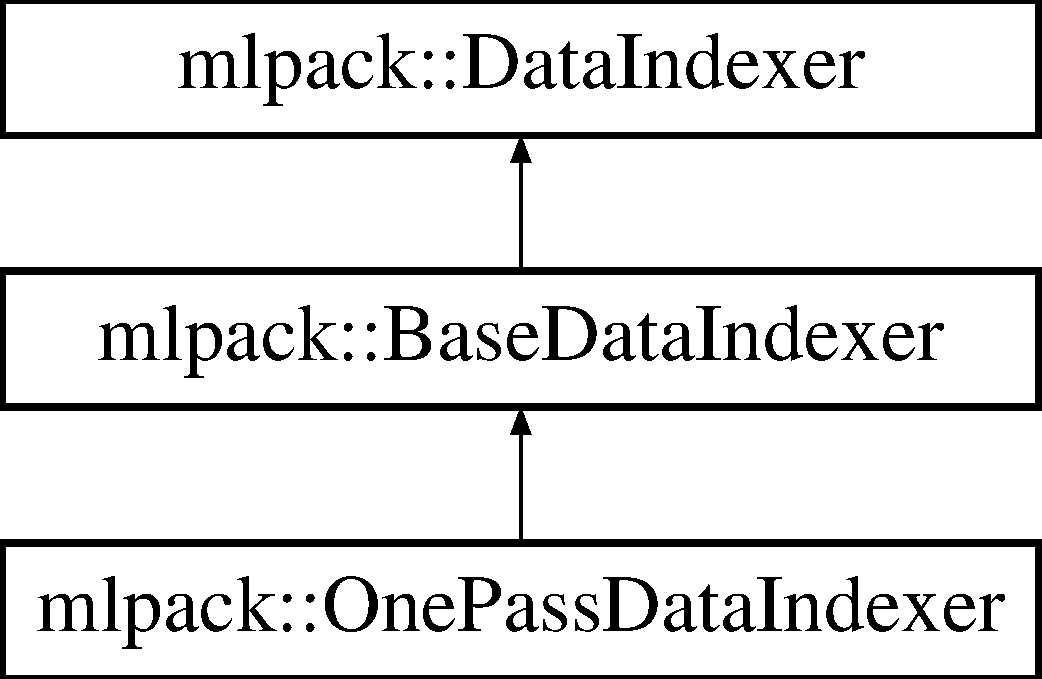
\includegraphics[height=3.000000cm]{classmlpack_1_1_base_data_indexer}
\end{center}
\end{figure}
\subsection*{Public Member Functions}
\begin{DoxyCompactItemize}
\item 
\hypertarget{classmlpack_1_1_base_data_indexer_a6542ba9420fbf16b258f533ad7feeafb}{
EventSpace {\bfseries contexts} ()}
\label{classmlpack_1_1_base_data_indexer_a6542ba9420fbf16b258f533ad7feeafb}

\item 
\hypertarget{classmlpack_1_1_base_data_indexer_a68b3500567d2ce7454da5ab64f80ff41}{
vector$<$ string $>$ {\bfseries pred\_\-labels} ()}
\label{classmlpack_1_1_base_data_indexer_a68b3500567d2ce7454da5ab64f80ff41}

\item 
\hypertarget{classmlpack_1_1_base_data_indexer_a82868b102570634a7b352f8d2b94b46e}{
vector$<$ string $>$ {\bfseries outcome\_\-labels} ()}
\label{classmlpack_1_1_base_data_indexer_a82868b102570634a7b352f8d2b94b46e}

\item 
\hypertarget{classmlpack_1_1_base_data_indexer_a968875f8d7cd612ff458f331cc263b8e}{
vector$<$ int $>$ {\bfseries pred\_\-counts} ()}
\label{classmlpack_1_1_base_data_indexer_a968875f8d7cd612ff458f331cc263b8e}

\item 
\hypertarget{classmlpack_1_1_base_data_indexer_a359a04d8614a211c06e4bfd4b752a027}{
int {\bfseries num\_\-events} ()}
\label{classmlpack_1_1_base_data_indexer_a359a04d8614a211c06e4bfd4b752a027}

\end{DoxyCompactItemize}
\subsection*{Protected Member Functions}
\begin{DoxyCompactItemize}
\item 
\hypertarget{classmlpack_1_1_base_data_indexer_adff552c54379efa08d23d21ea170f7e8}{
int {\bfseries sort\_\-n\_\-merge} (EventSpace elist, bool s)}
\label{classmlpack_1_1_base_data_indexer_adff552c54379efa08d23d21ea170f7e8}

\item 
\hypertarget{classmlpack_1_1_base_data_indexer_aad9a6ca736ededac457b7f706085d71f}{
void {\bfseries update} (\hyperlink{structmlpack_1_1_feature_set}{FeatureSet} context, map$<$ string, int $>$ \&pred\_\-index, map$<$ string, int $>$ \&counter, int cutoff)}
\label{classmlpack_1_1_base_data_indexer_aad9a6ca736ededac457b7f706085d71f}

\end{DoxyCompactItemize}
\subsection*{Protected Attributes}
\begin{DoxyCompactItemize}
\item 
\hypertarget{classmlpack_1_1_base_data_indexer_a6f1f70488b08e36dbca9c8e169dd0eac}{
EventSpace {\bfseries events}}
\label{classmlpack_1_1_base_data_indexer_a6f1f70488b08e36dbca9c8e169dd0eac}

\item 
\hypertarget{classmlpack_1_1_base_data_indexer_ac5e15e4a1bd23097dc69735c22c3b0b3}{
vector$<$ string $>$ {\bfseries plabels}}
\label{classmlpack_1_1_base_data_indexer_ac5e15e4a1bd23097dc69735c22c3b0b3}

\item 
\hypertarget{classmlpack_1_1_base_data_indexer_a03fe152079ac7f7651481574c56e9966}{
vector$<$ string $>$ {\bfseries olabels}}
\label{classmlpack_1_1_base_data_indexer_a03fe152079ac7f7651481574c56e9966}

\item 
\hypertarget{classmlpack_1_1_base_data_indexer_a931a85f90cfc730447468a0bae76ea01}{
vector$<$ int $>$ {\bfseries pcounts}}
\label{classmlpack_1_1_base_data_indexer_a931a85f90cfc730447468a0bae76ea01}

\item 
\hypertarget{classmlpack_1_1_base_data_indexer_a6ff416d6739c46e1bd76df92e2a5c2b3}{
int {\bfseries n\_\-events}}
\label{classmlpack_1_1_base_data_indexer_a6ff416d6739c46e1bd76df92e2a5c2b3}

\end{DoxyCompactItemize}


The documentation for this class was generated from the following file:\begin{DoxyCompactItemize}
\item 
include/mlpack/index.hpp\end{DoxyCompactItemize}

\hypertarget{classmlpack_1_1_data_indexer}{
\section{mlpack::DataIndexer Class Reference}
\label{classmlpack_1_1_data_indexer}\index{mlpack::DataIndexer@{mlpack::DataIndexer}}
}
Inheritance diagram for mlpack::DataIndexer:\begin{figure}[H]
\begin{center}
\leavevmode
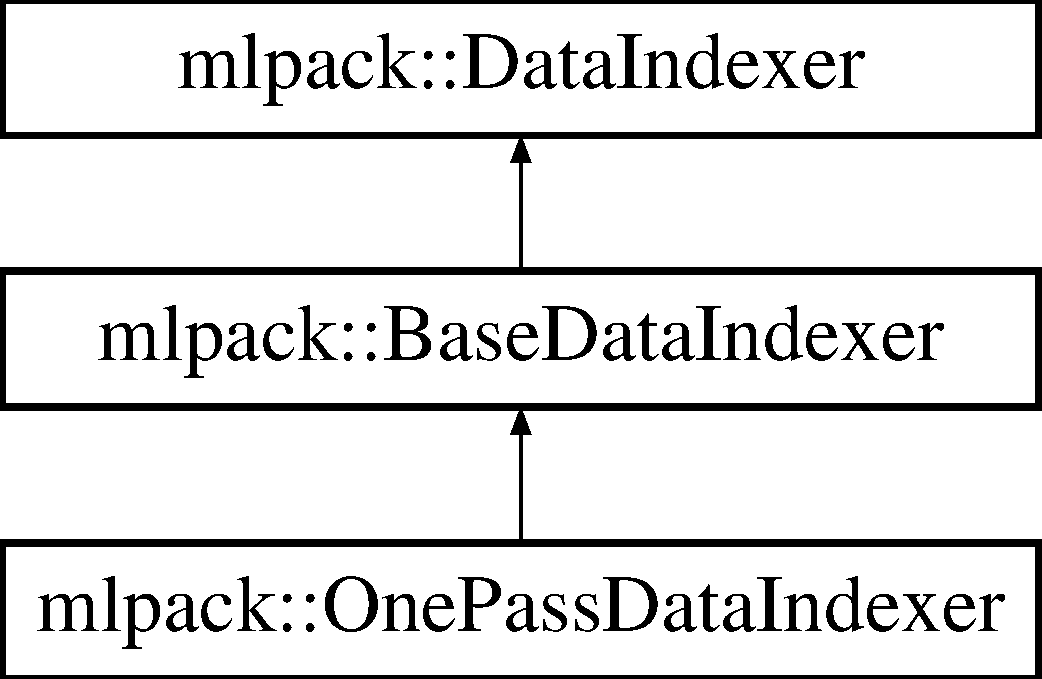
\includegraphics[height=3.000000cm]{classmlpack_1_1_data_indexer}
\end{center}
\end{figure}
\subsection*{Public Member Functions}
\begin{DoxyCompactItemize}
\item 
\hypertarget{classmlpack_1_1_data_indexer_a6a7edec1bed416e1efd71a23bcb2599a}{
virtual EventSpace {\bfseries contexts} ()=0}
\label{classmlpack_1_1_data_indexer_a6a7edec1bed416e1efd71a23bcb2599a}

\item 
\hypertarget{classmlpack_1_1_data_indexer_a5692f64eefc9003101f3b45d8d20472b}{
virtual vector$<$ string $>$ {\bfseries pred\_\-labels} ()=0}
\label{classmlpack_1_1_data_indexer_a5692f64eefc9003101f3b45d8d20472b}

\item 
\hypertarget{classmlpack_1_1_data_indexer_ab2f0529ade1a9f59e7d39d3da05eccb5}{
virtual vector$<$ int $>$ {\bfseries pred\_\-counts} ()=0}
\label{classmlpack_1_1_data_indexer_ab2f0529ade1a9f59e7d39d3da05eccb5}

\item 
\hypertarget{classmlpack_1_1_data_indexer_afa962d995218071829ec21cac917170c}{
virtual vector$<$ string $>$ {\bfseries outcome\_\-labels} ()=0}
\label{classmlpack_1_1_data_indexer_afa962d995218071829ec21cac917170c}

\item 
\hypertarget{classmlpack_1_1_data_indexer_a003cb740715f17db9c988eef0923f94a}{
virtual int {\bfseries num\_\-events} ()=0}
\label{classmlpack_1_1_data_indexer_a003cb740715f17db9c988eef0923f94a}

\end{DoxyCompactItemize}


The documentation for this class was generated from the following file:\begin{DoxyCompactItemize}
\item 
include/mlpack/index.hpp\end{DoxyCompactItemize}

\hypertarget{structmlpack_1_1_event}{
\section{mlpack::Event Struct Reference}
\label{structmlpack_1_1_event}\index{mlpack::Event@{mlpack::Event}}
}


{\ttfamily \#include $<$events.hpp$>$}

\subsection*{Public Member Functions}
\begin{DoxyCompactItemize}
\item 
\hypertarget{structmlpack_1_1_event_a59ebb3e8400d4849b8397b346ea4dee3}{
{\bfseries Event} (\hyperlink{structmlpack_1_1_feature_set}{FeatureSet} f, string o, int c)}
\label{structmlpack_1_1_event_a59ebb3e8400d4849b8397b346ea4dee3}

\end{DoxyCompactItemize}
\subsection*{Public Attributes}
\begin{DoxyCompactItemize}
\item 
\hypertarget{structmlpack_1_1_event_a755f573108dc50b1124cfba4c2a2c96c}{
\hyperlink{structmlpack_1_1_feature_set}{FeatureSet} {\bfseries context}}
\label{structmlpack_1_1_event_a755f573108dc50b1124cfba4c2a2c96c}

\item 
\hypertarget{structmlpack_1_1_event_a9f4cfe705671f5dfbe787a5dd2df4c24}{
string {\bfseries outcome}}
\label{structmlpack_1_1_event_a9f4cfe705671f5dfbe787a5dd2df4c24}

\item 
\hypertarget{structmlpack_1_1_event_ab33c2416b182e31f40f1be1542be9f74}{
int {\bfseries count}}
\label{structmlpack_1_1_event_ab33c2416b182e31f40f1be1542be9f74}

\item 
\hypertarget{structmlpack_1_1_event_ad81581cf10f9f431e062d98ee1239d33}{
int {\bfseries oid}}
\label{structmlpack_1_1_event_ad81581cf10f9f431e062d98ee1239d33}

\end{DoxyCompactItemize}


\subsection{Detailed Description}
For representing an event instance in the training data. An event consists of an outcome and a list of features (context). 

The documentation for this struct was generated from the following file:\begin{DoxyCompactItemize}
\item 
include/mlpack/events.hpp\end{DoxyCompactItemize}

\hypertarget{classmlpack_1_1_event_stream}{
\section{mlpack::EventStream Class Reference}
\label{classmlpack_1_1_event_stream}\index{mlpack::EventStream@{mlpack::EventStream}}
}


{\ttfamily \#include $<$events.hpp$>$}

Inheritance diagram for mlpack::EventStream:\begin{figure}[H]
\begin{center}
\leavevmode
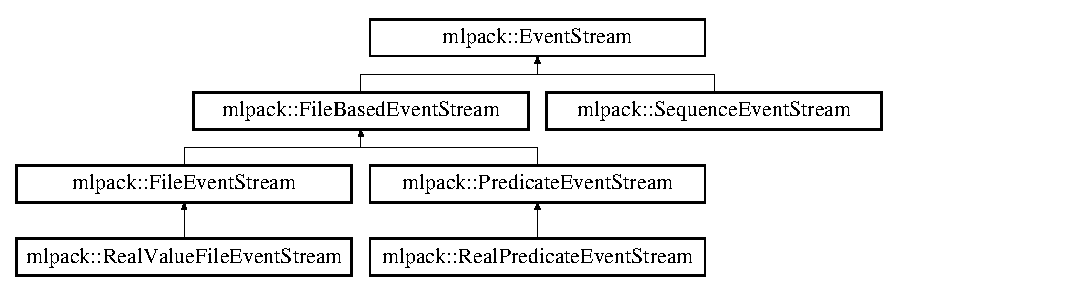
\includegraphics[height=3.472868cm]{classmlpack_1_1_event_stream}
\end{center}
\end{figure}
\subsection*{Public Member Functions}
\begin{DoxyCompactItemize}
\item 
\hypertarget{classmlpack_1_1_event_stream_aa3b7f54240069f28f60d3e99b125f990}{
virtual \hyperlink{structmlpack_1_1_event}{Event} {\bfseries next} ()=0}
\label{classmlpack_1_1_event_stream_aa3b7f54240069f28f60d3e99b125f990}

\item 
\hypertarget{classmlpack_1_1_event_stream_ae53414a60c19d80291d9f76168160497}{
virtual bool {\bfseries has\_\-next} ()=0}
\label{classmlpack_1_1_event_stream_ae53414a60c19d80291d9f76168160497}

\end{DoxyCompactItemize}


\subsection{Detailed Description}
Represents a stream of events, used to read events to the indexer. 

The documentation for this class was generated from the following file:\begin{DoxyCompactItemize}
\item 
include/mlpack/events.hpp\end{DoxyCompactItemize}

\hypertarget{structmlpack_1_1_feature}{
\section{mlpack::Feature Struct Reference}
\label{structmlpack_1_1_feature}\index{mlpack::Feature@{mlpack::Feature}}
}
\subsection*{Public Member Functions}
\begin{DoxyCompactItemize}
\item 
\hypertarget{structmlpack_1_1_feature_af731a0d0274d23be34feeadbbecbf5fb}{
{\bfseries Feature} (string n, double v)}
\label{structmlpack_1_1_feature_af731a0d0274d23be34feeadbbecbf5fb}

\end{DoxyCompactItemize}
\subsection*{Public Attributes}
\begin{DoxyCompactItemize}
\item 
\hypertarget{structmlpack_1_1_feature_a0e4f86f38cc28733574e4a8a60d71de8}{
string {\bfseries name}}
\label{structmlpack_1_1_feature_a0e4f86f38cc28733574e4a8a60d71de8}

\item 
\hypertarget{structmlpack_1_1_feature_af60cfe02f10b9555df297816e45fb267}{
double {\bfseries value}}
\label{structmlpack_1_1_feature_af60cfe02f10b9555df297816e45fb267}

\item 
\hypertarget{structmlpack_1_1_feature_a60a991b860b743263e0b4ce1fe57e093}{
int {\bfseries id}}
\label{structmlpack_1_1_feature_a60a991b860b743263e0b4ce1fe57e093}

\end{DoxyCompactItemize}


The documentation for this struct was generated from the following file:\begin{DoxyCompactItemize}
\item 
include/mlpack/feature.hpp\end{DoxyCompactItemize}

\hypertarget{structmlpack_1_1_feature_set}{
\section{mlpack::FeatureSet Struct Reference}
\label{structmlpack_1_1_feature_set}\index{mlpack::FeatureSet@{mlpack::FeatureSet}}
}
\subsection*{Public Member Functions}
\begin{DoxyCompactItemize}
\item 
\hypertarget{structmlpack_1_1_feature_set_a7ddcbd5e1cd3cc2395ca5cef9884fbda}{
void {\bfseries put} (\hyperlink{structmlpack_1_1_feature}{Feature} feat)}
\label{structmlpack_1_1_feature_set_a7ddcbd5e1cd3cc2395ca5cef9884fbda}

\item 
\hypertarget{structmlpack_1_1_feature_set_a478c03c6f3111ad4e43f18bab61dbea8}{
\hyperlink{structmlpack_1_1_feature}{Feature} {\bfseries get} (string name)}
\label{structmlpack_1_1_feature_set_a478c03c6f3111ad4e43f18bab61dbea8}

\item 
\hypertarget{structmlpack_1_1_feature_set_afc59ed95c07ebee674ff57dd793897bd}{
FeatureIterator {\bfseries begin} ()}
\label{structmlpack_1_1_feature_set_afc59ed95c07ebee674ff57dd793897bd}

\item 
\hypertarget{structmlpack_1_1_feature_set_a28c6f535c55cfc2411594a1c04ffd4b8}{
FeatureIterator {\bfseries end} ()}
\label{structmlpack_1_1_feature_set_a28c6f535c55cfc2411594a1c04ffd4b8}

\item 
\hypertarget{structmlpack_1_1_feature_set_a03f6ef5d3ed15477f6be98b00d6bc3bd}{
FeatureIterator {\bfseries find} (string name)}
\label{structmlpack_1_1_feature_set_a03f6ef5d3ed15477f6be98b00d6bc3bd}

\item 
\hypertarget{structmlpack_1_1_feature_set_a3ede7a822cc52868f47a3b68f1bb3737}{
size\_\-t {\bfseries size} ()}
\label{structmlpack_1_1_feature_set_a3ede7a822cc52868f47a3b68f1bb3737}

\end{DoxyCompactItemize}
\subsection*{Public Attributes}
\begin{DoxyCompactItemize}
\item 
\hypertarget{structmlpack_1_1_feature_set_a60be60b4b309eb16b09e8459ac8414d2}{
FeatureMap {\bfseries feat\_\-map}}
\label{structmlpack_1_1_feature_set_a60be60b4b309eb16b09e8459ac8414d2}

\end{DoxyCompactItemize}


The documentation for this struct was generated from the following file:\begin{DoxyCompactItemize}
\item 
include/mlpack/feature.hpp\end{DoxyCompactItemize}

\hypertarget{classmlpack_1_1_file_based_event_stream}{
\section{mlpack::FileBasedEventStream Class Reference}
\label{classmlpack_1_1_file_based_event_stream}\index{mlpack::FileBasedEventStream@{mlpack::FileBasedEventStream}}
}
Inheritance diagram for mlpack::FileBasedEventStream:\begin{figure}[H]
\begin{center}
\leavevmode
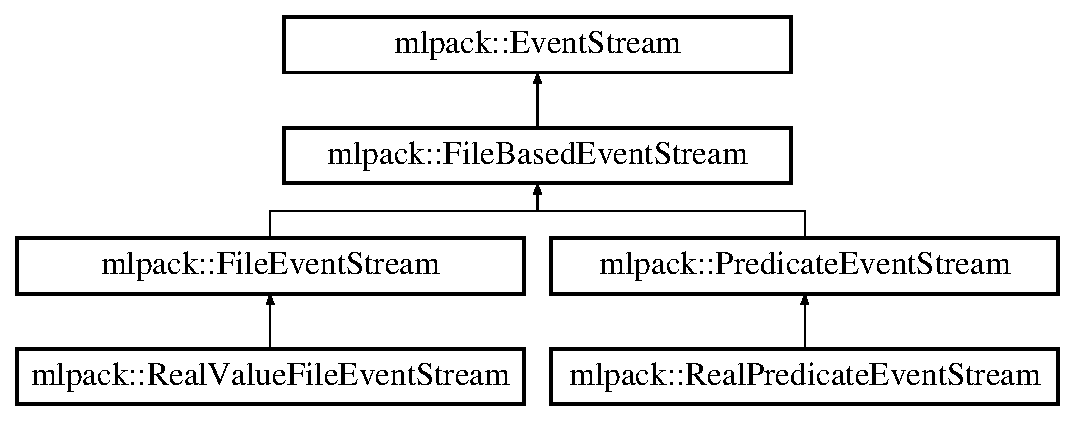
\includegraphics[height=4.000000cm]{classmlpack_1_1_file_based_event_stream}
\end{center}
\end{figure}
\subsection*{Public Member Functions}
\begin{DoxyCompactItemize}
\item 
\hypertarget{classmlpack_1_1_file_based_event_stream_ae3c00550fbb7b7cd18e62d9ba2863714}{
{\bfseries FileBasedEventStream} (string fname)}
\label{classmlpack_1_1_file_based_event_stream_ae3c00550fbb7b7cd18e62d9ba2863714}

\item 
\hypertarget{classmlpack_1_1_file_based_event_stream_a5f791d0f78009b477d219928a6cb19d7}{
virtual \hyperlink{structmlpack_1_1_event}{Event} {\bfseries next} ()}
\label{classmlpack_1_1_file_based_event_stream_a5f791d0f78009b477d219928a6cb19d7}

\item 
\hypertarget{classmlpack_1_1_file_based_event_stream_a826d8e9828bfe2d67e698e7782f8044c}{
bool {\bfseries has\_\-next} ()}
\label{classmlpack_1_1_file_based_event_stream_a826d8e9828bfe2d67e698e7782f8044c}

\end{DoxyCompactItemize}
\subsection*{Protected Attributes}
\begin{DoxyCompactItemize}
\item 
\hypertarget{classmlpack_1_1_file_based_event_stream_ad5b84711ba9ad5c66db5b454452b9ed7}{
ifstream {\bfseries input}}
\label{classmlpack_1_1_file_based_event_stream_ad5b84711ba9ad5c66db5b454452b9ed7}

\item 
\hypertarget{classmlpack_1_1_file_based_event_stream_a1b6d8662fa3aab1e5647d14b59186127}{
string {\bfseries line}}
\label{classmlpack_1_1_file_based_event_stream_a1b6d8662fa3aab1e5647d14b59186127}

\end{DoxyCompactItemize}


The documentation for this class was generated from the following file:\begin{DoxyCompactItemize}
\item 
include/mlpack/events.hpp\end{DoxyCompactItemize}

\hypertarget{classmlpack_1_1_file_event_stream}{
\section{mlpack::FileEventStream Class Reference}
\label{classmlpack_1_1_file_event_stream}\index{mlpack::FileEventStream@{mlpack::FileEventStream}}
}
Inheritance diagram for mlpack::FileEventStream:\begin{figure}[H]
\begin{center}
\leavevmode
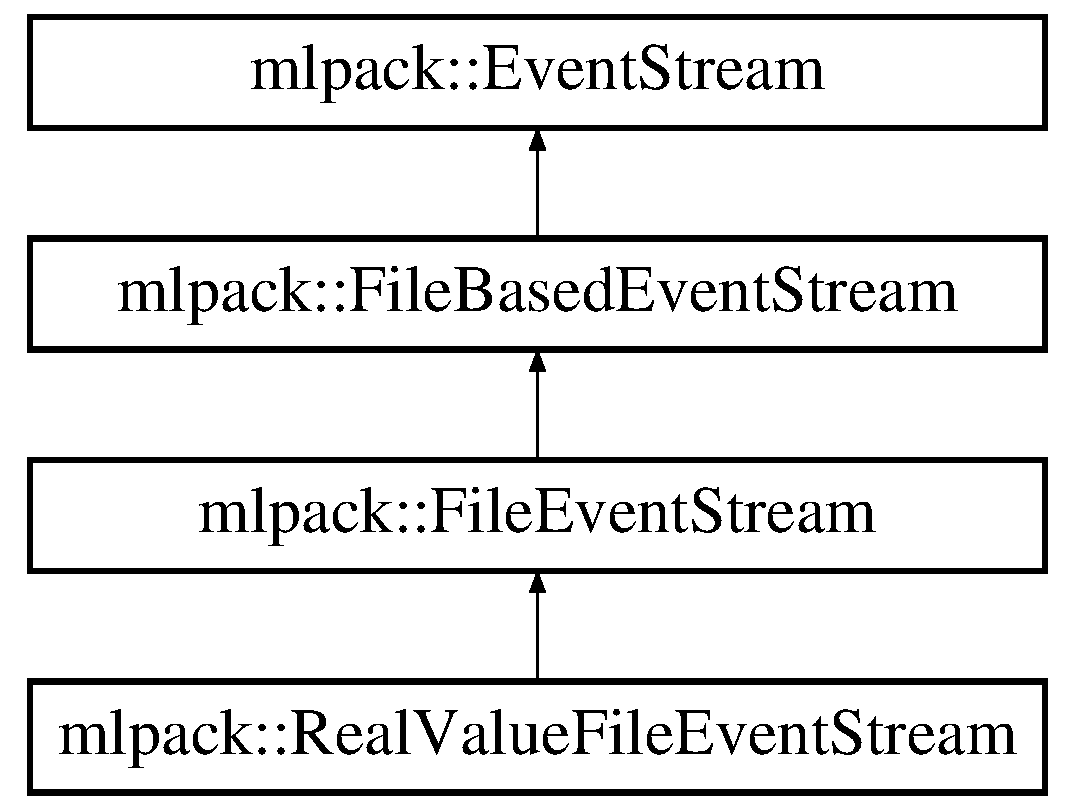
\includegraphics[height=4.000000cm]{classmlpack_1_1_file_event_stream}
\end{center}
\end{figure}
\subsection*{Public Member Functions}
\begin{DoxyCompactItemize}
\item 
\hypertarget{classmlpack_1_1_file_event_stream_ab4fdb0b43ef647c62888d583210a4f40}{
{\bfseries FileEventStream} (string fname)}
\label{classmlpack_1_1_file_event_stream_ab4fdb0b43ef647c62888d583210a4f40}

\item 
\hypertarget{classmlpack_1_1_file_event_stream_a13a65fd63969c2e662d3eec17df57edf}{
\hyperlink{structmlpack_1_1_event}{Event} {\bfseries next} ()}
\label{classmlpack_1_1_file_event_stream_a13a65fd63969c2e662d3eec17df57edf}

\end{DoxyCompactItemize}


The documentation for this class was generated from the following file:\begin{DoxyCompactItemize}
\item 
include/mlpack/events.hpp\end{DoxyCompactItemize}

\hypertarget{classmlpack_1_1_g_i_s_model}{
\section{mlpack::GISModel Class Reference}
\label{classmlpack_1_1_g_i_s_model}\index{mlpack::GISModel@{mlpack::GISModel}}
}
Inheritance diagram for mlpack::GISModel:\begin{figure}[H]
\begin{center}
\leavevmode
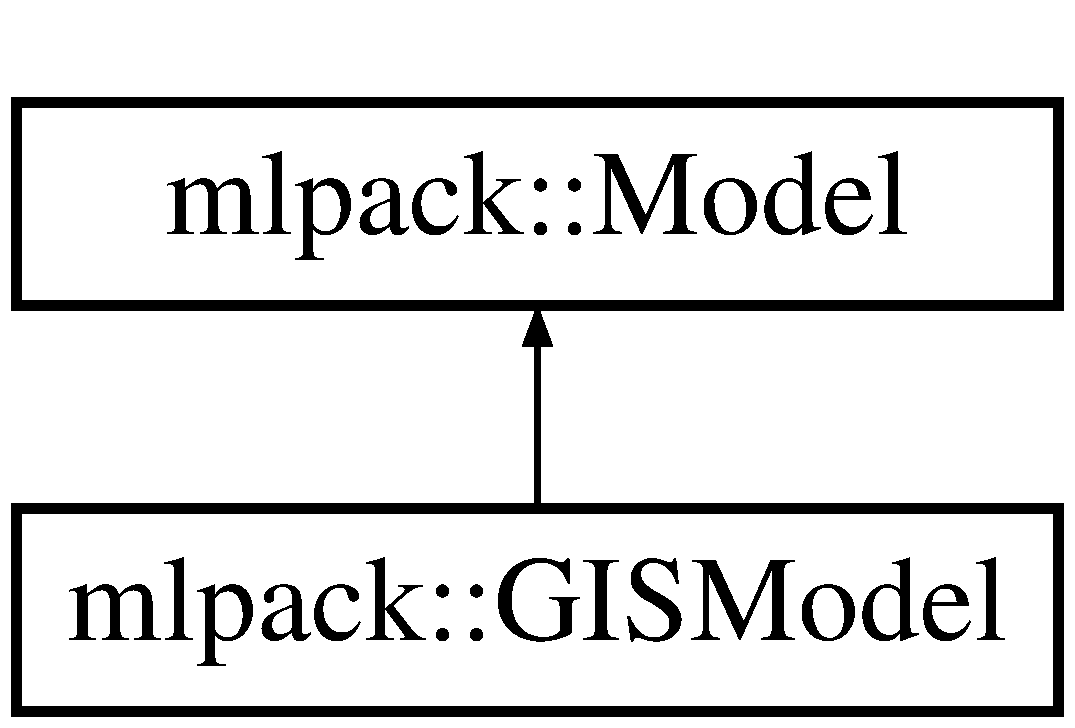
\includegraphics[height=2.000000cm]{classmlpack_1_1_g_i_s_model}
\end{center}
\end{figure}
\subsection*{Public Member Functions}
\begin{DoxyCompactItemize}
\item 
\hypertarget{classmlpack_1_1_g_i_s_model_a70b5617bb746965a114ce53f40994f97}{
{\bfseries GISModel} (vector$<$ \hyperlink{classmlpack_1_1_parameters}{Parameters} $>$ params, vector$<$ string $>$ pls, vector$<$ string $>$ ols, \hyperlink{classmlpack_1_1_prior}{Prior} $\ast$p)}
\label{classmlpack_1_1_g_i_s_model_a70b5617bb746965a114ce53f40994f97}

\item 
\hypertarget{classmlpack_1_1_g_i_s_model_a20df804c3af48f04a5064b01121eb241}{
vector$<$ double $>$ {\bfseries eval} (\hyperlink{structmlpack_1_1_feature_set}{FeatureSet} context)}
\label{classmlpack_1_1_g_i_s_model_a20df804c3af48f04a5064b01121eb241}

\item 
\hypertarget{classmlpack_1_1_g_i_s_model_ae231a7276c7b42cf82205570c1d6ecd9}{
string {\bfseries best\_\-outcome} (vector$<$ double $>$ outcomes)}
\label{classmlpack_1_1_g_i_s_model_ae231a7276c7b42cf82205570c1d6ecd9}

\item 
\hypertarget{classmlpack_1_1_g_i_s_model_a1c288157a87919c02c75cc7f3d60dca8}{
string {\bfseries outcome} (int i)}
\label{classmlpack_1_1_g_i_s_model_a1c288157a87919c02c75cc7f3d60dca8}

\item 
\hypertarget{classmlpack_1_1_g_i_s_model_afa224d21ba44eb9a5a47e2f9d75e0ad9}{
int {\bfseries index} (string out)}
\label{classmlpack_1_1_g_i_s_model_afa224d21ba44eb9a5a47e2f9d75e0ad9}

\item 
\hypertarget{classmlpack_1_1_g_i_s_model_a6a7fe5c4c7d8808cdaa55ad793135872}{
int {\bfseries pred\_\-index} (string pred)}
\label{classmlpack_1_1_g_i_s_model_a6a7fe5c4c7d8808cdaa55ad793135872}

\end{DoxyCompactItemize}
\subsection*{Static Public Member Functions}
\begin{DoxyCompactItemize}
\item 
\hypertarget{classmlpack_1_1_g_i_s_model_a9aa802dd7a6e98fe771cda2da611982c}{
static vector$<$ double $>$ {\bfseries eval} (\hyperlink{structmlpack_1_1_feature_set}{FeatureSet} context, vector$<$ double $>$ \&prior, \hyperlink{classmlpack_1_1_maxent_parameters}{MaxentParameters} model)}
\label{classmlpack_1_1_g_i_s_model_a9aa802dd7a6e98fe771cda2da611982c}

\end{DoxyCompactItemize}
\subsection*{Protected Attributes}
\begin{DoxyCompactItemize}
\item 
\hypertarget{classmlpack_1_1_g_i_s_model_a1f75f3fbb76b7e38ed81f5a1b9387d1e}{
vector$<$ string $>$ {\bfseries olabels}}
\label{classmlpack_1_1_g_i_s_model_a1f75f3fbb76b7e38ed81f5a1b9387d1e}

\item 
\hypertarget{classmlpack_1_1_g_i_s_model_a610ca84b801a2a91d63374b2d0d8871b}{
map$<$ string, int $>$ {\bfseries pmap}}
\label{classmlpack_1_1_g_i_s_model_a610ca84b801a2a91d63374b2d0d8871b}

\item 
\hypertarget{classmlpack_1_1_g_i_s_model_ae9f9e8d5dab18d55bd90d2afb0b4d487}{
\hyperlink{classmlpack_1_1_maxent_parameters}{MaxentParameters} $\ast$ {\bfseries maxent\_\-params}}
\label{classmlpack_1_1_g_i_s_model_ae9f9e8d5dab18d55bd90d2afb0b4d487}

\item 
\hypertarget{classmlpack_1_1_g_i_s_model_a9a2e28ae8bc7f625aeda3985d660d716}{
\hyperlink{classmlpack_1_1_prior}{Prior} $\ast$ {\bfseries prior}}
\label{classmlpack_1_1_g_i_s_model_a9a2e28ae8bc7f625aeda3985d660d716}

\end{DoxyCompactItemize}
\subsection*{Friends}
\begin{DoxyCompactItemize}
\item 
\hypertarget{classmlpack_1_1_g_i_s_model_ac98d07dd8f7b70e16ccb9a01abf56b9c}{
class {\bfseries boost::serialization::access}}
\label{classmlpack_1_1_g_i_s_model_ac98d07dd8f7b70e16ccb9a01abf56b9c}

\end{DoxyCompactItemize}


The documentation for this class was generated from the following file:\begin{DoxyCompactItemize}
\item 
include/mlpack/model.hpp\end{DoxyCompactItemize}

\hypertarget{classmlpack_1_1_g_i_s_trainer}{
\section{mlpack::GISTrainer Class Reference}
\label{classmlpack_1_1_g_i_s_trainer}\index{mlpack::GISTrainer@{mlpack::GISTrainer}}
}
Inheritance diagram for mlpack::GISTrainer:\begin{figure}[H]
\begin{center}
\leavevmode
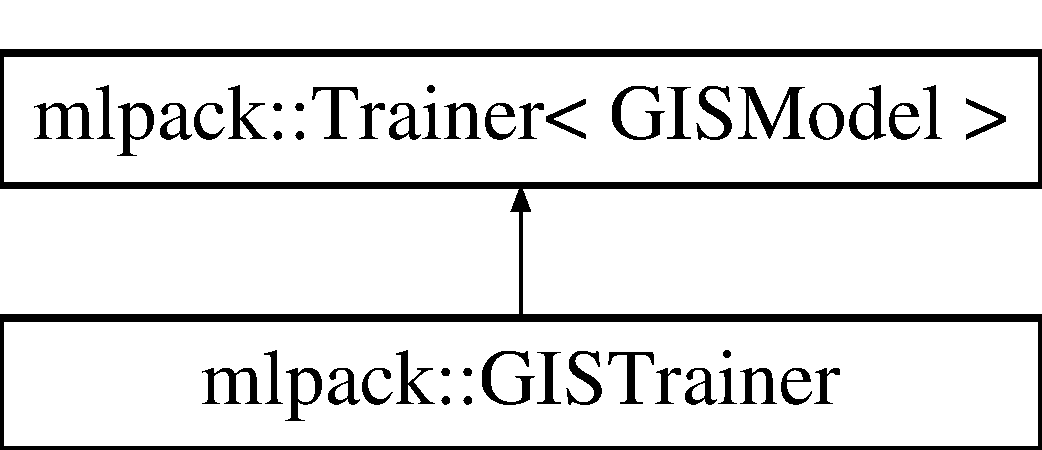
\includegraphics[height=2.000000cm]{classmlpack_1_1_g_i_s_trainer}
\end{center}
\end{figure}
\subsection*{Public Member Functions}
\begin{DoxyCompactItemize}
\item 
\hypertarget{classmlpack_1_1_g_i_s_trainer_a57f2a11dfa5ae1a08044cd9e5319c216}{
\hyperlink{classmlpack_1_1_g_i_s_model}{GISModel} {\bfseries train} (\hyperlink{classmlpack_1_1_data_indexer}{DataIndexer} \&di, \hyperlink{classmlpack_1_1_prior}{Prior} $\ast$prior, ptree config)}
\label{classmlpack_1_1_g_i_s_trainer_a57f2a11dfa5ae1a08044cd9e5319c216}

\end{DoxyCompactItemize}


The documentation for this class was generated from the following file:\begin{DoxyCompactItemize}
\item 
include/mlpack/gistrainer.hpp\end{DoxyCompactItemize}

\hypertarget{classmlpack_1_1_maxent_parameters}{
\section{mlpack::MaxentParameters Class Reference}
\label{classmlpack_1_1_maxent_parameters}\index{mlpack::MaxentParameters@{mlpack::MaxentParameters}}
}
\subsection*{Public Member Functions}
\begin{DoxyCompactItemize}
\item 
\hypertarget{classmlpack_1_1_maxent_parameters_a8a2fefa3c44532441401a25a550dbcf1}{
{\bfseries MaxentParameters} (vector$<$ \hyperlink{classmlpack_1_1_parameters}{Parameters} $>$ ps, double corr\_\-p, double corr\_\-const, int n\_\-out)}
\label{classmlpack_1_1_maxent_parameters_a8a2fefa3c44532441401a25a550dbcf1}

\end{DoxyCompactItemize}
\subsection*{Public Attributes}
\begin{DoxyCompactItemize}
\item 
\hypertarget{classmlpack_1_1_maxent_parameters_a9c031c4f1ff7c16fcadedf18f97e4541}{
vector$<$ \hyperlink{classmlpack_1_1_parameters}{Parameters} $>$ {\bfseries params}}
\label{classmlpack_1_1_maxent_parameters_a9c031c4f1ff7c16fcadedf18f97e4541}

\item 
\hypertarget{classmlpack_1_1_maxent_parameters_a83832c17dd75a64680e3ec9b158ee066}{
int {\bfseries n\_\-outcomes}}
\label{classmlpack_1_1_maxent_parameters_a83832c17dd75a64680e3ec9b158ee066}

\item 
\hypertarget{classmlpack_1_1_maxent_parameters_adb77778a4f8f9b949b14067de6cb6d85}{
double {\bfseries corr\_\-constant}}
\label{classmlpack_1_1_maxent_parameters_adb77778a4f8f9b949b14067de6cb6d85}

\item 
\hypertarget{classmlpack_1_1_maxent_parameters_aaa904a124b94c2c1b0433b1721bd746c}{
double {\bfseries const\_\-inverse}}
\label{classmlpack_1_1_maxent_parameters_aaa904a124b94c2c1b0433b1721bd746c}

\item 
\hypertarget{classmlpack_1_1_maxent_parameters_a13d16c4a737d177f45f094b21fc173cf}{
double {\bfseries corr\_\-param}}
\label{classmlpack_1_1_maxent_parameters_a13d16c4a737d177f45f094b21fc173cf}

\end{DoxyCompactItemize}
\subsection*{Friends}
\begin{DoxyCompactItemize}
\item 
\hypertarget{classmlpack_1_1_maxent_parameters_ac98d07dd8f7b70e16ccb9a01abf56b9c}{
class {\bfseries boost::serialization::access}}
\label{classmlpack_1_1_maxent_parameters_ac98d07dd8f7b70e16ccb9a01abf56b9c}

\end{DoxyCompactItemize}


The documentation for this class was generated from the following file:\begin{DoxyCompactItemize}
\item 
include/mlpack/params.hpp\end{DoxyCompactItemize}

\hypertarget{classmlpack_1_1_model}{
\section{mlpack::Model Class Reference}
\label{classmlpack_1_1_model}\index{mlpack::Model@{mlpack::Model}}
}
Inheritance diagram for mlpack::Model:\begin{figure}[H]
\begin{center}
\leavevmode
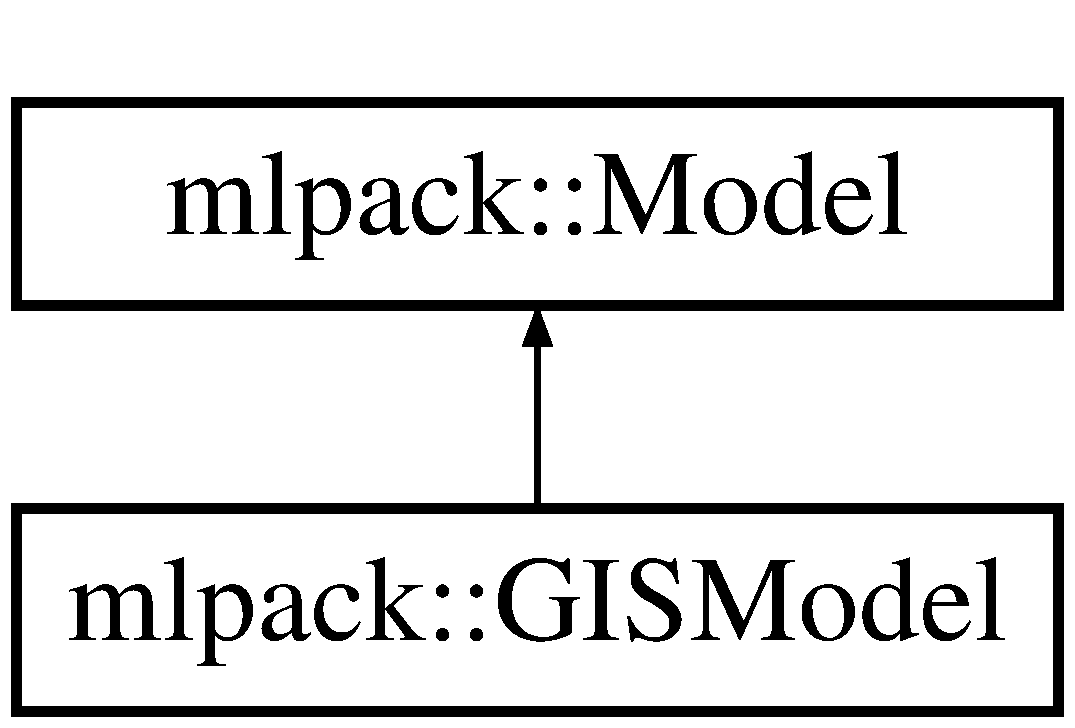
\includegraphics[height=2.000000cm]{classmlpack_1_1_model}
\end{center}
\end{figure}
\subsection*{Public Member Functions}
\begin{DoxyCompactItemize}
\item 
\hypertarget{classmlpack_1_1_model_a62004f99ecc70455338ccf206533787b}{
virtual vector$<$ double $>$ {\bfseries eval} (\hyperlink{structmlpack_1_1_feature_set}{FeatureSet} context)=0}
\label{classmlpack_1_1_model_a62004f99ecc70455338ccf206533787b}

\item 
\hypertarget{classmlpack_1_1_model_a6c991c3a264b14cc7ba25ccaba07017d}{
virtual string {\bfseries best\_\-outcome} (vector$<$ double $>$ outcomes)=0}
\label{classmlpack_1_1_model_a6c991c3a264b14cc7ba25ccaba07017d}

\item 
\hypertarget{classmlpack_1_1_model_a2dd8ed20b28dcbfd157d5d0a2cae4585}{
virtual string {\bfseries outcome} (int i)=0}
\label{classmlpack_1_1_model_a2dd8ed20b28dcbfd157d5d0a2cae4585}

\item 
\hypertarget{classmlpack_1_1_model_a6f9e4c74633a589343031571c0fc7db9}{
virtual int {\bfseries index} (string out)=0}
\label{classmlpack_1_1_model_a6f9e4c74633a589343031571c0fc7db9}

\item 
\hypertarget{classmlpack_1_1_model_a188aad4207f178e2ff01ca018df35471}{
virtual int {\bfseries pred\_\-index} (string pred)=0}
\label{classmlpack_1_1_model_a188aad4207f178e2ff01ca018df35471}

\end{DoxyCompactItemize}
\subsection*{Friends}
\begin{DoxyCompactItemize}
\item 
\hypertarget{classmlpack_1_1_model_ac98d07dd8f7b70e16ccb9a01abf56b9c}{
class {\bfseries boost::serialization::access}}
\label{classmlpack_1_1_model_ac98d07dd8f7b70e16ccb9a01abf56b9c}

\end{DoxyCompactItemize}


The documentation for this class was generated from the following file:\begin{DoxyCompactItemize}
\item 
include/mlpack/model.hpp\end{DoxyCompactItemize}

\hypertarget{classmlpack_1_1_one_pass_data_indexer}{
\section{mlpack::OnePassDataIndexer Class Reference}
\label{classmlpack_1_1_one_pass_data_indexer}\index{mlpack::OnePassDataIndexer@{mlpack::OnePassDataIndexer}}
}
Inheritance diagram for mlpack::OnePassDataIndexer:\begin{figure}[H]
\begin{center}
\leavevmode
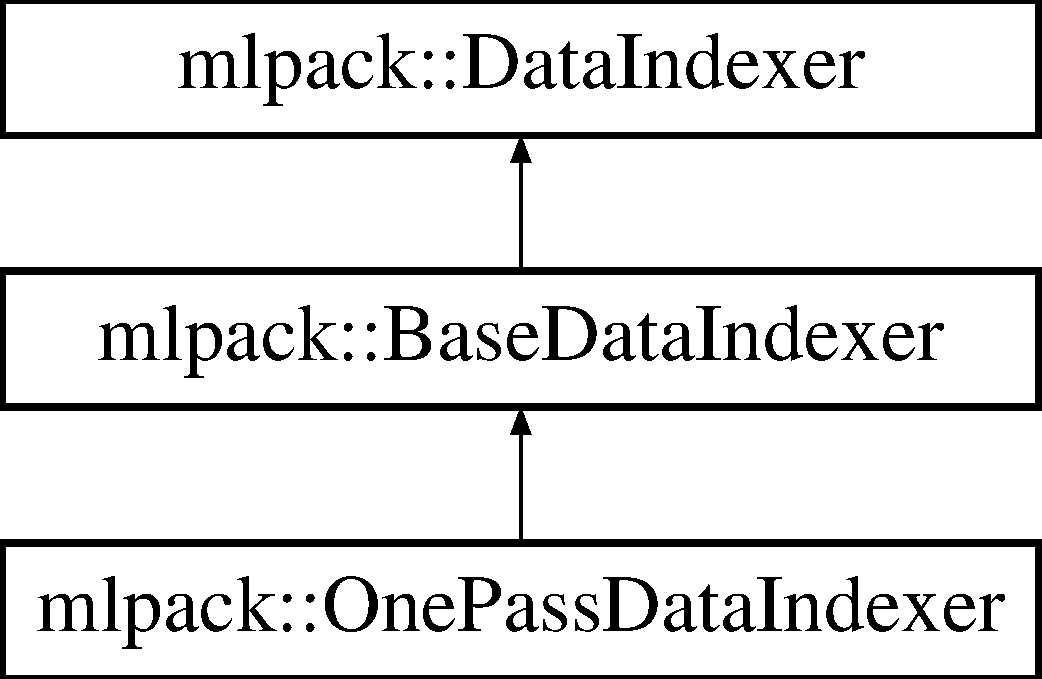
\includegraphics[height=3.000000cm]{classmlpack_1_1_one_pass_data_indexer}
\end{center}
\end{figure}
\subsection*{Public Member Functions}
\begin{DoxyCompactItemize}
\item 
\hypertarget{classmlpack_1_1_one_pass_data_indexer_a8e9d977e6781271f9f7ca0da2ce1bbd3}{
{\bfseries OnePassDataIndexer} (\hyperlink{classmlpack_1_1_event_stream}{EventStream} \&stream, int cutoff=0, bool \_\-sort=true)}
\label{classmlpack_1_1_one_pass_data_indexer_a8e9d977e6781271f9f7ca0da2ce1bbd3}

\end{DoxyCompactItemize}


The documentation for this class was generated from the following file:\begin{DoxyCompactItemize}
\item 
include/mlpack/index.hpp\end{DoxyCompactItemize}

\hypertarget{classmlpack_1_1_parameters}{
\section{mlpack::Parameters Class Reference}
\label{classmlpack_1_1_parameters}\index{mlpack::Parameters@{mlpack::Parameters}}
}
\subsection*{Public Member Functions}
\begin{DoxyCompactItemize}
\item 
\hypertarget{classmlpack_1_1_parameters_a3b1607f330f62f352670a1eade883afa}{
{\bfseries Parameters} (vector$<$ double $>$ ps, vector$<$ int $>$ os)}
\label{classmlpack_1_1_parameters_a3b1607f330f62f352670a1eade883afa}

\item 
\hypertarget{classmlpack_1_1_parameters_af513fa33bf660fd0d9183f758c11ee28}{
void {\bfseries set} (int oi, double param)}
\label{classmlpack_1_1_parameters_af513fa33bf660fd0d9183f758c11ee28}

\item 
\hypertarget{classmlpack_1_1_parameters_aebf0fb11b56c77a449e4b6088acc9d98}{
void {\bfseries update} (int oi, double param)}
\label{classmlpack_1_1_parameters_aebf0fb11b56c77a449e4b6088acc9d98}

\item 
\hypertarget{classmlpack_1_1_parameters_a2e1515cb0149f5cd94789d0dc11862be}{
void {\bfseries print} ()}
\label{classmlpack_1_1_parameters_a2e1515cb0149f5cd94789d0dc11862be}

\end{DoxyCompactItemize}
\subsection*{Public Attributes}
\begin{DoxyCompactItemize}
\item 
\hypertarget{classmlpack_1_1_parameters_af31dff55c545ca31a9c81b6b07508829}{
vector$<$ double $>$ {\bfseries params}}
\label{classmlpack_1_1_parameters_af31dff55c545ca31a9c81b6b07508829}

\item 
\hypertarget{classmlpack_1_1_parameters_ad23ef76f46921512d9a9dc6b3630884c}{
vector$<$ int $>$ {\bfseries outcomes}}
\label{classmlpack_1_1_parameters_ad23ef76f46921512d9a9dc6b3630884c}

\end{DoxyCompactItemize}
\subsection*{Friends}
\begin{DoxyCompactItemize}
\item 
\hypertarget{classmlpack_1_1_parameters_ac98d07dd8f7b70e16ccb9a01abf56b9c}{
class {\bfseries boost::serialization::access}}
\label{classmlpack_1_1_parameters_ac98d07dd8f7b70e16ccb9a01abf56b9c}

\end{DoxyCompactItemize}


The documentation for this class was generated from the following file:\begin{DoxyCompactItemize}
\item 
include/mlpack/params.hpp\end{DoxyCompactItemize}

\hypertarget{classmlpack_1_1_predicate_event_stream}{
\section{mlpack::PredicateEventStream Class Reference}
\label{classmlpack_1_1_predicate_event_stream}\index{mlpack::PredicateEventStream@{mlpack::PredicateEventStream}}
}
Inheritance diagram for mlpack::PredicateEventStream:\begin{figure}[H]
\begin{center}
\leavevmode
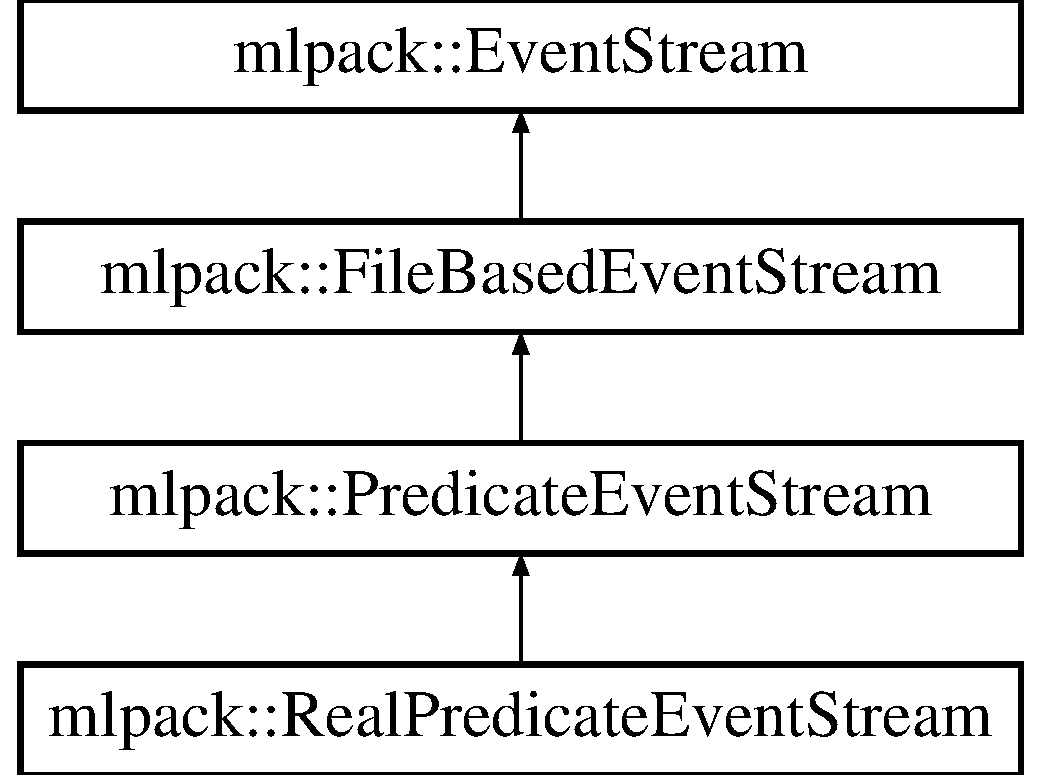
\includegraphics[height=4.000000cm]{classmlpack_1_1_predicate_event_stream}
\end{center}
\end{figure}
\subsection*{Public Member Functions}
\begin{DoxyCompactItemize}
\item 
\hypertarget{classmlpack_1_1_predicate_event_stream_ae4b2e2633ba3a789500abf1eb3787c9b}{
{\bfseries PredicateEventStream} (string fname)}
\label{classmlpack_1_1_predicate_event_stream_ae4b2e2633ba3a789500abf1eb3787c9b}

\item 
\hypertarget{classmlpack_1_1_predicate_event_stream_affb1a6e31e9ab7d68167f357c37e6b1b}{
\hyperlink{structmlpack_1_1_event}{Event} {\bfseries next} ()}
\label{classmlpack_1_1_predicate_event_stream_affb1a6e31e9ab7d68167f357c37e6b1b}

\end{DoxyCompactItemize}


The documentation for this class was generated from the following file:\begin{DoxyCompactItemize}
\item 
include/mlpack/events.hpp\end{DoxyCompactItemize}

\hypertarget{classmlpack_1_1_prior}{
\section{mlpack::Prior Class Reference}
\label{classmlpack_1_1_prior}\index{mlpack::Prior@{mlpack::Prior}}
}
Inheritance diagram for mlpack::Prior:\begin{figure}[H]
\begin{center}
\leavevmode
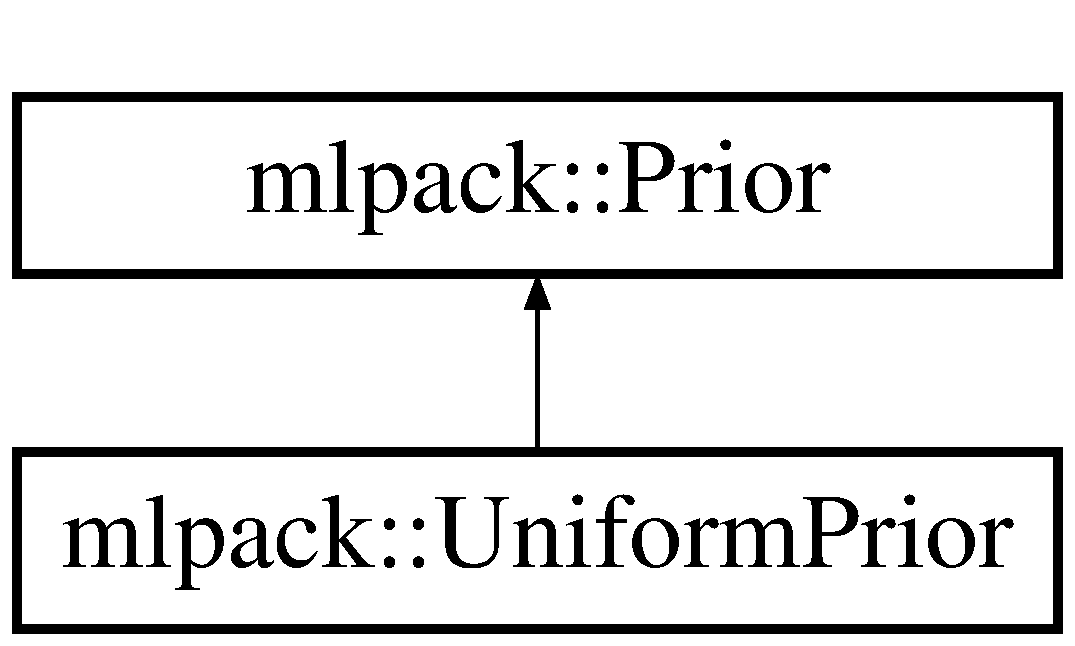
\includegraphics[height=2.000000cm]{classmlpack_1_1_prior}
\end{center}
\end{figure}
\subsection*{Public Member Functions}
\begin{DoxyCompactItemize}
\item 
\hypertarget{classmlpack_1_1_prior_a77157f8dde683313d7a0872e5f4204f1}{
virtual void {\bfseries log\_\-prior} (vector$<$ double $>$ \&dist, \hyperlink{structmlpack_1_1_feature_set}{FeatureSet} \&context)=0}
\label{classmlpack_1_1_prior_a77157f8dde683313d7a0872e5f4204f1}

\item 
\hypertarget{classmlpack_1_1_prior_a3e1b4e2bcc76dd9a5cfb213dedca9e5f}{
virtual void {\bfseries set\_\-labels} (vector$<$ string $>$ outcome\_\-labels, vector$<$ string $>$ pred\_\-labels)=0}
\label{classmlpack_1_1_prior_a3e1b4e2bcc76dd9a5cfb213dedca9e5f}

\end{DoxyCompactItemize}
\subsection*{Friends}
\begin{DoxyCompactItemize}
\item 
\hypertarget{classmlpack_1_1_prior_ac98d07dd8f7b70e16ccb9a01abf56b9c}{
class {\bfseries boost::serialization::access}}
\label{classmlpack_1_1_prior_ac98d07dd8f7b70e16ccb9a01abf56b9c}

\end{DoxyCompactItemize}


The documentation for this class was generated from the following file:\begin{DoxyCompactItemize}
\item 
include/mlpack/prior.hpp\end{DoxyCompactItemize}

\hypertarget{classmlpack_1_1_real_predicate_event_stream}{
\section{mlpack::RealPredicateEventStream Class Reference}
\label{classmlpack_1_1_real_predicate_event_stream}\index{mlpack::RealPredicateEventStream@{mlpack::RealPredicateEventStream}}
}
Inheritance diagram for mlpack::RealPredicateEventStream:\begin{figure}[H]
\begin{center}
\leavevmode
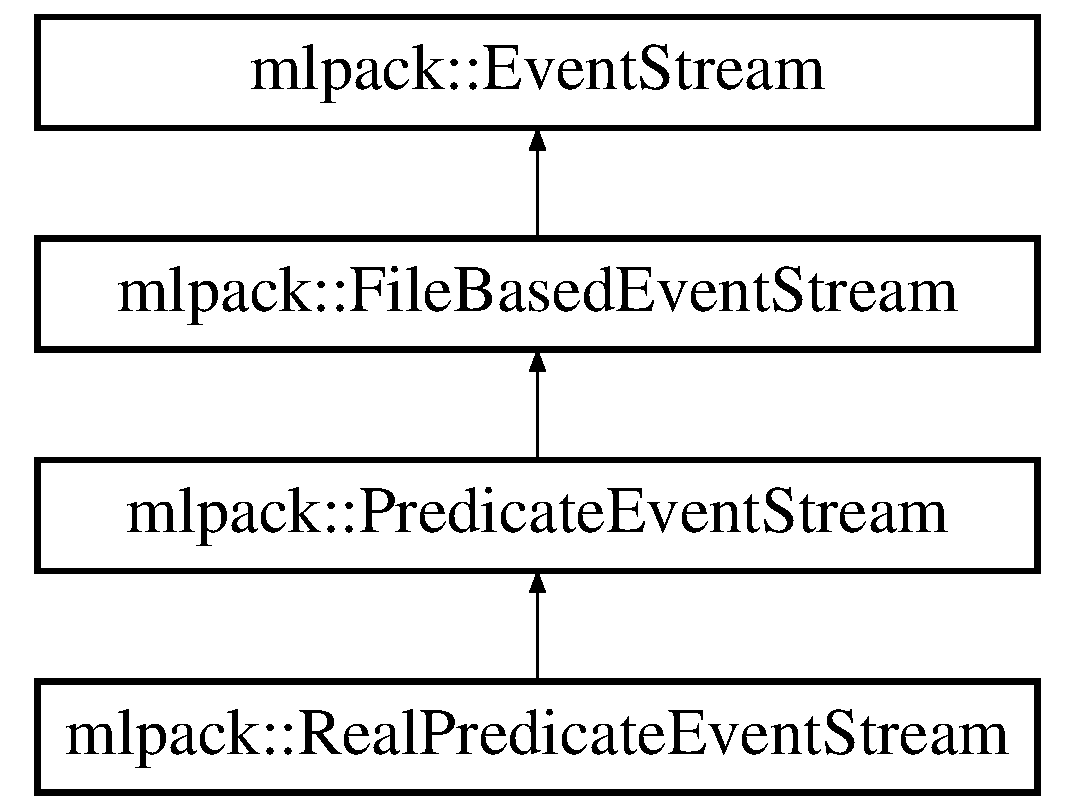
\includegraphics[height=4.000000cm]{classmlpack_1_1_real_predicate_event_stream}
\end{center}
\end{figure}
\subsection*{Public Member Functions}
\begin{DoxyCompactItemize}
\item 
\hypertarget{classmlpack_1_1_real_predicate_event_stream_a11fa52e766139624bd415f81bcd0a0b9}{
{\bfseries RealPredicateEventStream} (string fname)}
\label{classmlpack_1_1_real_predicate_event_stream_a11fa52e766139624bd415f81bcd0a0b9}

\item 
\hypertarget{classmlpack_1_1_real_predicate_event_stream_aa2677da8e06cfe3d0c60aaf82eaf9cca}{
\hyperlink{structmlpack_1_1_event}{Event} {\bfseries next} ()}
\label{classmlpack_1_1_real_predicate_event_stream_aa2677da8e06cfe3d0c60aaf82eaf9cca}

\end{DoxyCompactItemize}


The documentation for this class was generated from the following file:\begin{DoxyCompactItemize}
\item 
include/mlpack/events.hpp\end{DoxyCompactItemize}

\hypertarget{classmlpack_1_1_real_value_file_event_stream}{
\section{mlpack::RealValueFileEventStream Class Reference}
\label{classmlpack_1_1_real_value_file_event_stream}\index{mlpack::RealValueFileEventStream@{mlpack::RealValueFileEventStream}}
}
Inheritance diagram for mlpack::RealValueFileEventStream:\begin{figure}[H]
\begin{center}
\leavevmode
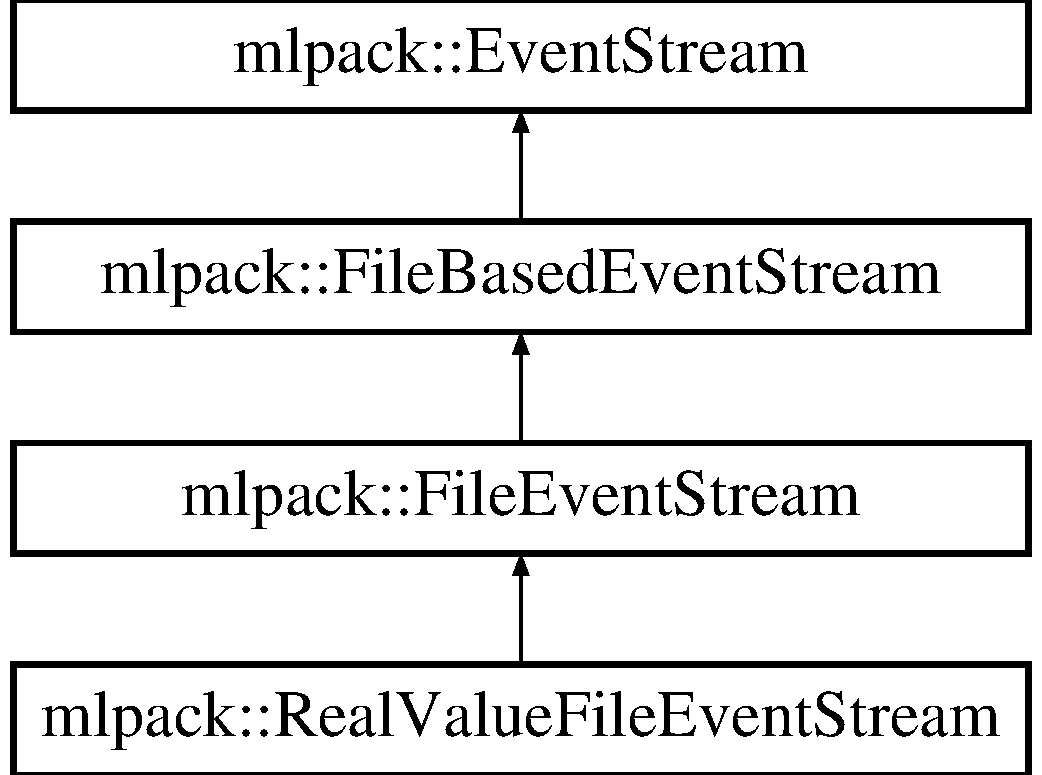
\includegraphics[height=4.000000cm]{classmlpack_1_1_real_value_file_event_stream}
\end{center}
\end{figure}
\subsection*{Public Member Functions}
\begin{DoxyCompactItemize}
\item 
\hypertarget{classmlpack_1_1_real_value_file_event_stream_a1fef86991b34d2425cbbd7fea9d86da4}{
{\bfseries RealValueFileEventStream} (string fname)}
\label{classmlpack_1_1_real_value_file_event_stream_a1fef86991b34d2425cbbd7fea9d86da4}

\item 
\hypertarget{classmlpack_1_1_real_value_file_event_stream_abe8738da0cba6334ab463d2d9b660f52}{
\hyperlink{structmlpack_1_1_event}{Event} {\bfseries next} ()}
\label{classmlpack_1_1_real_value_file_event_stream_abe8738da0cba6334ab463d2d9b660f52}

\end{DoxyCompactItemize}


The documentation for this class was generated from the following file:\begin{DoxyCompactItemize}
\item 
include/mlpack/events.hpp\end{DoxyCompactItemize}

\hypertarget{classmlpack_1_1_sequence_event_stream}{
\section{mlpack::SequenceEventStream Class Reference}
\label{classmlpack_1_1_sequence_event_stream}\index{mlpack::SequenceEventStream@{mlpack::SequenceEventStream}}
}
Inheritance diagram for mlpack::SequenceEventStream:\begin{figure}[H]
\begin{center}
\leavevmode
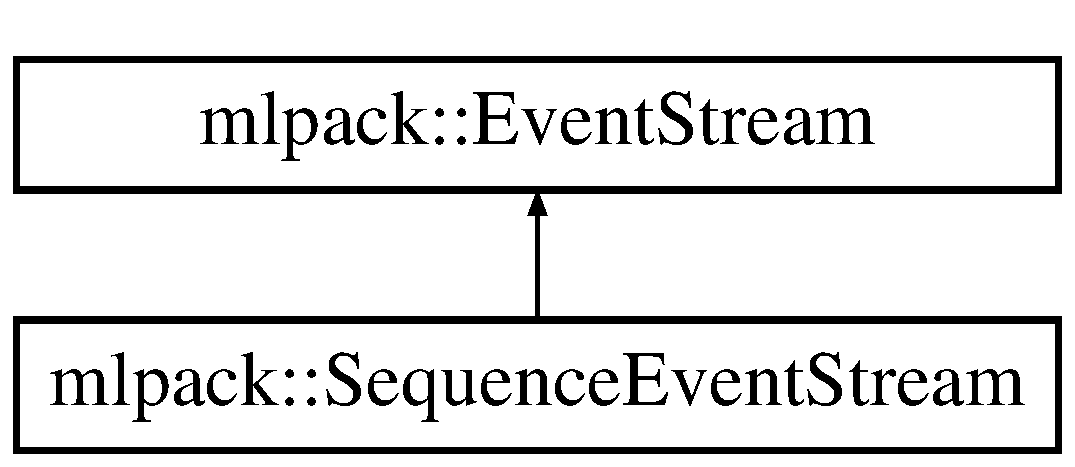
\includegraphics[height=2.000000cm]{classmlpack_1_1_sequence_event_stream}
\end{center}
\end{figure}
\subsection*{Public Member Functions}
\begin{DoxyCompactItemize}
\item 
\hypertarget{classmlpack_1_1_sequence_event_stream_ae6422ba56e4c8f84960c74c2bee8f757}{
void {\bfseries add\_\-event} (\hyperlink{structmlpack_1_1_event}{Event} ev)}
\label{classmlpack_1_1_sequence_event_stream_ae6422ba56e4c8f84960c74c2bee8f757}

\item 
\hypertarget{classmlpack_1_1_sequence_event_stream_aabea2d7fea55cf3d755d8ee6829470c0}{
\hyperlink{structmlpack_1_1_event}{Event} {\bfseries next} ()}
\label{classmlpack_1_1_sequence_event_stream_aabea2d7fea55cf3d755d8ee6829470c0}

\item 
\hypertarget{classmlpack_1_1_sequence_event_stream_ac4e3f481db6538917745f4cd99722ec1}{
bool {\bfseries has\_\-next} ()}
\label{classmlpack_1_1_sequence_event_stream_ac4e3f481db6538917745f4cd99722ec1}

\end{DoxyCompactItemize}
\subsection*{Protected Attributes}
\begin{DoxyCompactItemize}
\item 
\hypertarget{classmlpack_1_1_sequence_event_stream_ad88d2af30e2d8e5beced9467e4146722}{
EventSpace {\bfseries events}}
\label{classmlpack_1_1_sequence_event_stream_ad88d2af30e2d8e5beced9467e4146722}

\item 
\hypertarget{classmlpack_1_1_sequence_event_stream_a1641e54080e52343acc5ae0a36c20ba7}{
EventSpace::iterator {\bfseries eit}}
\label{classmlpack_1_1_sequence_event_stream_a1641e54080e52343acc5ae0a36c20ba7}

\end{DoxyCompactItemize}


The documentation for this class was generated from the following file:\begin{DoxyCompactItemize}
\item 
include/mlpack/events.hpp\end{DoxyCompactItemize}

\hypertarget{classmlpack_1_1_trainer}{
\section{mlpack::Trainer$<$ T $>$ Class Template Reference}
\label{classmlpack_1_1_trainer}\index{mlpack::Trainer@{mlpack::Trainer}}
}
\subsection*{Public Member Functions}
\begin{DoxyCompactItemize}
\item 
\hypertarget{classmlpack_1_1_trainer_a30d68e9ccf847d21b03c00e0be79cc55}{
virtual T {\bfseries train} (\hyperlink{classmlpack_1_1_data_indexer}{DataIndexer} \&di, \hyperlink{classmlpack_1_1_prior}{Prior} $\ast$prior, ptree config)=0}
\label{classmlpack_1_1_trainer_a30d68e9ccf847d21b03c00e0be79cc55}

\end{DoxyCompactItemize}
\subsubsection*{template$<$typename T$>$ class mlpack::Trainer$<$ T $>$}



The documentation for this class was generated from the following file:\begin{DoxyCompactItemize}
\item 
include/mlpack/trainer.hpp\end{DoxyCompactItemize}

\hypertarget{classmlpack_1_1_uniform_prior}{
\section{mlpack::UniformPrior Class Reference}
\label{classmlpack_1_1_uniform_prior}\index{mlpack::UniformPrior@{mlpack::UniformPrior}}
}
Inheritance diagram for mlpack::UniformPrior:\begin{figure}[H]
\begin{center}
\leavevmode
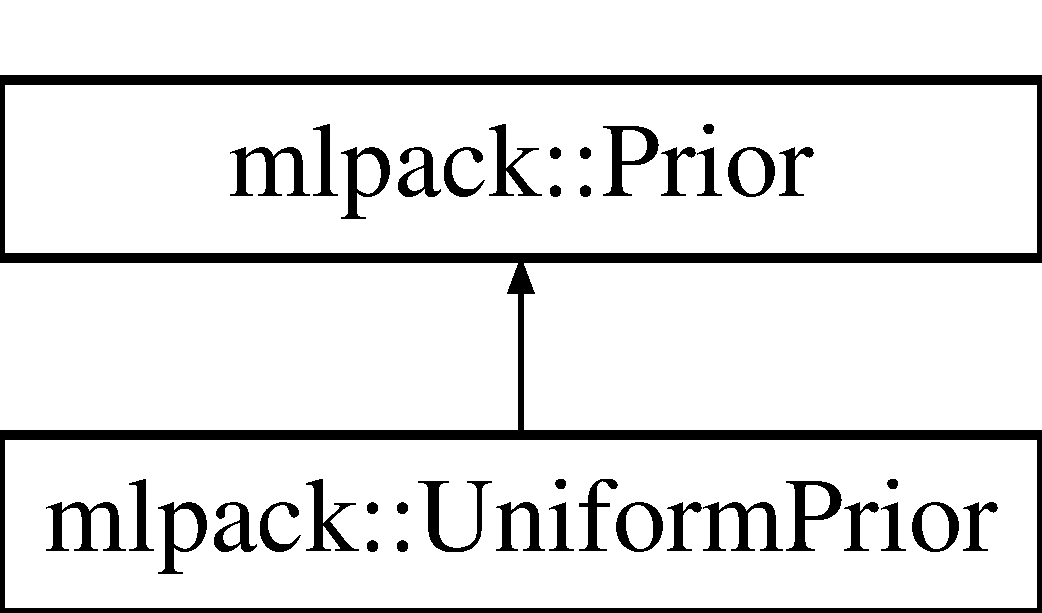
\includegraphics[height=2.000000cm]{classmlpack_1_1_uniform_prior}
\end{center}
\end{figure}
\subsection*{Public Member Functions}
\begin{DoxyCompactItemize}
\item 
\hypertarget{classmlpack_1_1_uniform_prior_a2c449695fbb3005563e3898dd578239c}{
void {\bfseries log\_\-prior} (vector$<$ double $>$ \&dist, \hyperlink{structmlpack_1_1_feature_set}{FeatureSet} \&context)}
\label{classmlpack_1_1_uniform_prior_a2c449695fbb3005563e3898dd578239c}

\item 
\hypertarget{classmlpack_1_1_uniform_prior_ac6dbf3c0036c3da9549e7923b6e86f61}{
void {\bfseries set\_\-labels} (vector$<$ string $>$ outcome\_\-labels, vector$<$ string $>$ pred\_\-labels)}
\label{classmlpack_1_1_uniform_prior_ac6dbf3c0036c3da9549e7923b6e86f61}

\end{DoxyCompactItemize}
\subsection*{Public Attributes}
\begin{DoxyCompactItemize}
\item 
\hypertarget{classmlpack_1_1_uniform_prior_a0879fed0e11bea4b5e64b7d5620ab360}{
int {\bfseries n\_\-outcomes}}
\label{classmlpack_1_1_uniform_prior_a0879fed0e11bea4b5e64b7d5620ab360}

\item 
\hypertarget{classmlpack_1_1_uniform_prior_abdad93d521111dc6b8b9928b0dd286d0}{
double {\bfseries r}}
\label{classmlpack_1_1_uniform_prior_abdad93d521111dc6b8b9928b0dd286d0}

\end{DoxyCompactItemize}
\subsection*{Friends}
\begin{DoxyCompactItemize}
\item 
\hypertarget{classmlpack_1_1_uniform_prior_ac98d07dd8f7b70e16ccb9a01abf56b9c}{
class {\bfseries boost::serialization::access}}
\label{classmlpack_1_1_uniform_prior_ac98d07dd8f7b70e16ccb9a01abf56b9c}

\end{DoxyCompactItemize}


The documentation for this class was generated from the following file:\begin{DoxyCompactItemize}
\item 
include/mlpack/prior.hpp\end{DoxyCompactItemize}

\printindex
\end{document}
